\documentclass[times, utf8, zavrsni, numeric]{fer}
\usepackage{booktabs}
\usepackage{graphicx}
\usepackage{wrapfig}

\graphicspath{{./images/}}

\begin{document}

\thesisnumber{6651}

\title{Rendering of Voxelized Space with Vulkan Using Hardware Accelerated Ray Tracing}

\author{Ivan Karlović}

\maketitle

% Ispis stranice s napomenom o umetanju izvornika rada. Uklonite naredbu \izvornik ako želite izbaciti tu stranicu.
\izvornik

% Dodavanje zahvale ili prazne stranice. Ako ne želite dodati zahvalu, naredbu ostavite radi prazne stranice.
\zahvala{}

\tableofcontents

\chapter{Introduction}

Ever since OpenGL 1.0 was released in 1992., the computer hardware industry has been continuously improving on what GPUs are capable of. Today's graphics cards are boasting FP performance of over 10 TFLOPS, making them more than $10^{12}$ times faster than the ones initially released with OpenGL 1.0. While OpenGL has changed over the last 20 years (current version 4.6), it can no longer extract the full potential of the graphics cards built with modern architectures. This is why Vulkan was created, a new API designed from ground up for the modern GPU architectures. It is a more advanced API, leaving more control in the hands of the application, whereas in OpenGL a lot of operations were handled by the GPU drivers.

Modern graphics cards have reached another important milestone within the last few years. While realtime rendering has been done almost exclusively using rasterization, it has now become possible to render significant parts of the scene using ray tracing, such as shadow, reflection and global illumination. There are implementations today that even render the whole scene solely using ray tracing. A whole new pipeline has been created for modern graphic APIs (including Vulkan) that can utilize hardware to accelerate certain aspects of ray tracing, most notably ray triangle intersections. This paper will first explore how to efficiently represent voxelized space on the GPU and then render it using the new ray tracing pipeline.

\chapter{Used tools and technologies}
\section{C++}

\begin{center}
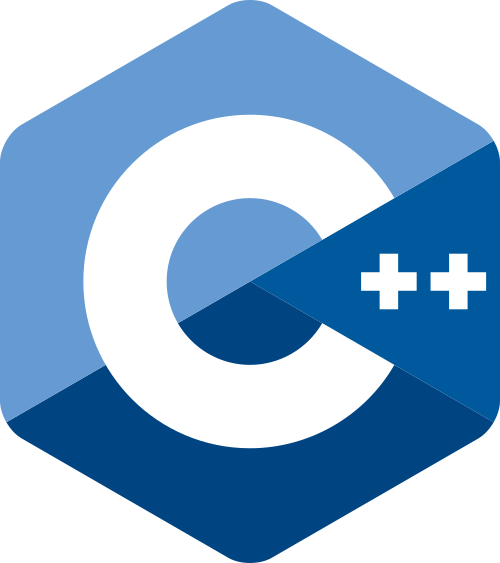
\includegraphics[width=0.1\textwidth]{cpp_logo.png}
\end{center}

C++ is a primarily object-oriented programming language. It was developed by Bjarne Stroustrup as an extension of the C language and was initially standardized by ISO in 1998, the current standard being C++17. Due to its speed and low-level memory management capabilities, it became the first choice for the development of 3D applications.

\section{Vulkan}

\begin{center}

\includegraphics[width=0.6\textwidth]{vulkan_logo.png}
\end{center}

Vulkan \cite{vulkan_spec} is a graphics API released on 26th of February 2016 by the Khronos consortium, an open industry consortium consisting of over 150 software and hardware companies. It's a cross-platform graphics and compute API which is constantly being worked and expanded upon. The current version, and the one used in this paper, is 1.2. While it’s capable of better utilizing the GPU resources, it’s not meant as a replacement for OpenGL which still works very well for most use cases. In Vulkan however, the application has a lot more control (and by extent, responsibility) over the application. A lot of features and functions that were handled and synchronized by the driver are now up to the application to deal with and control.

Vulkan is released as a C99 header file. Since its initial release, more than several different bindings for various languages have been created, including the ones for C++, C\#, Python, Java, Haskell and many others. There even exists a binding that allows for Direct3D 9 applications to run over Vulkan.

Along with Vulkan, a new standard for programmable shaders was developed, SPIR-V. It can be compiled from GLSL (and recently HLSL) source code ensuring more precise interpretation of the specification, addressing many issues that stemmed from GLSL and HLSL shaders behaving differently on different vendor hardware.

Throught this paper, Vulkan 1.2.141 used via C++ bindings.

\section{LunarG SDK}

\begin{center}

\includegraphics[width=0.2\textwidth]{lunarg_logo.png}
\end{center}

LunarG SDK is a Windows and Linux compatible Vulkan SDK which provides the various components need to develop a Vulkan application, including Vulkan loader, Vulkan layers, debugging tools, SPIR-V tools, Vulkan runtime installer, documentation samples and demos.

\section{GLFW}
GLFW is a Graphics Library FrameWork originally developed for OpenGL. It a simple API that today supports Vulkan that is used for creating windows and surfaces, as well as receiving inputs and events.

\section{Optix denoiser}
Optix denoiser \cite{nvidia_optix} is a part of the Nvidia Optix SDK that can be used standalone. It takes noisy images produced by ray tracing and outputs a denoised image. While there exists a more advanced variant that takes two additional images - one representing the albedo colour of each fragment and the other with the normal of each fragment, it isn't used in this paper.

\chapter{Representation of voxelized space using greedy meshing}

\chapter{What is ray tracing and how it compares to rasterization}
\section{Rasterization overview}

\section{Ray tracing algorithm}

\chapter{Overview of Vulkan and its ray tracing extension}
While OpenGL is still continuously being updated, there is only so much that can be done for an API that is almost three decades old. This is why Vulkan was created, designed from the ground up with the modern architecture of graphics cards in mind. It's a cross-platform graphics and compute API that can run on a variety of operating systems and which many devices can support. Due to all of this, Vulkan is a complex and extremely verbose API. While on the surface it might look like it's a lot more complex than OpenGL, the difference I much smaller than it appears to be on the first glance. A lot of complexity (and verbosity) comes from the fact that a lot of responsibility (and by extension, control) has been shifted from the driver to the application.

As a result, a hello triangle program that might have taken 20 or so lines in OpenGL 1.0 now takes over 900 lines of code in Vulkan \cite{vulkan_tutorial}.

%Before continuing with ray tracing, it would be worth to first visit several recurring patterns which can be found when writing a Vulkan application, as well as generally describe the parts that are common to most graphical applications.

Several key points that make Vulkan more performant and more suitable for modern systems than OpenGL:
\begin{itemize}
	\item Low API overhead. Instead of issuing commands to the device one by one, multiple commands are recorded to command buffers which are then submitted to the GPU to be executed.
	\item API makes no guarantees on order of execution of commands recorded to the submitted command buffer. The application needs to use pipeline and memory barriers to create dependencies between commands. In a well-written application, this means that commands will only be blocked by the commands that they depend on.
	\item API has been written with multicore CPUs in mind. While it's not possible to concurrently record commands to the same command buffer from multiple threads, it is possible to create and (concurrently) record commands to secondary command buffers that can then be tied together in a primary command buffer.
	\item API controls memory allocations. In OpenGL, all device memory allocations have been managed by the driver, whereas in Vulkan all memory allocations need to be explicitly managed by the application.
	\item Most objects in the API are immutable. While this makes the API a bit more cumbersome to use, the driver can use this guarantee to make optimizations that weren't possible in OpenGL.
	\item Better debugging support. Vulkan introduces the concept of validation layers - layers that can be placed between the application and the driver to ensure that calls to the API are valid and well-formed.
\end{itemize}

\section{Vulkan model overview}
\subsection{Instance and device}
The first object to be created when using Vulkan is an instance (\texttt{vk::Instance}). The application can specify which version of the API will be used, as well as enable various validation layers. The instance is the closest thing in Vulkan to OpenGLs global state. Once the instance is created, various physical devices can be enumerated (\texttt{vk::PhysicalDevice}), each representing specific Vulkan-compatible devices connected to the system. They can be queried for their capabilities and various extension support. Next step is to create a logical device (\texttt{vk::Device}) based on one of the physical devices. From this point on, the logical device facilitates most of applications communication with the API.

\subsection{Queues and command buffers}
Most of communication between the application and the device is done with command pools (\texttt{vk::CommandPool}), command buffers (\texttt{vk::CommandBuffer}) and queues (\texttt{vk::Queue}). First, a command pool is created, connected to one of the queues available from the physical device. It's possible to then allocate one or more command buffers from this pool. Once the commands are recorded to the command buffer, it can be submitted to the queue for the device to execute it.

\subsection{Synchronization}
\subsubsection{Synchronization within buffers}
All of the commands in a command buffer are executed asynchronously. Pipeline barriers act as execution barriers between various commands, ensuring various commands are executed after described pipeline stages. Each pipeline barrier can hold a reference to one or more image and buffer memory barriers (\texttt{vk::ImageMemoryBarrier} and \texttt{vk::BufferMemoryBarrier}), determining the order of the operations over those resources (eg. preventing read operations on a buffer before all writes have been completed).

\subsubsection{Synchronization between buffers}
Submitting one command buffer before the other does not guarantee it will be executed first. On each command buffer submission, it's possible to supply one or more binary semaphores (\texttt{vk::Semaphore}) that the command buffer will wait on to be signalled before executing, or semaphores that will be signalled once the command buffer has completed its execution. Fences (\texttt{vk::Fence}) are used similarly, but they enable command buffer synchronization with the application (eg. waiting for an image to be rendered before attempting to present it on screen). In Vulkan 1.2, timeline semaphores have been introduced with the \texttt{VK\_KHR\_TIMELINE\_SEMAPHORE} extension. It enables more complex dependencies to be expressed with a single semaphore holding several points in time instead of being forced to use a binary semaphore between each of the steps.

\subsection{Memory management overview}
Every Vulkan object created by the application will have its own handle. Once an object is created, the application has to keep track of it and destroy it once it's no longer needed. Most Vulkan objects don't need additional memory other than its own metadata. The two exceptions are pooled resources and application managed resources.

\subsubsection{Pooled resources}
Two examples of pooled resources are descriptor sets and command buffers. First a pool object (\texttt{vk::DescriptorPool} and \texttt{vk::CommandPool}) needs to be created from which desired objects are then allocated. The memory of these pools is managed by the device driver.

\subsubsection{Application managed resources}
Two most notable entries of this category are buffers (\texttt{vk::Buffer}) and Images (\texttt{vk::Image}). Once a handle to one of these resources is created, the application must query for the memory requirements of the object and then allocate device memory (\texttt{DeviceMemory}) with suitable properties. Finally, this memory must then be bound to the object. It's recommended to allocate a single device memory and bind several objects to various offsets, especially since its possible to have only 4096 allocated device memory at one time (on Windows at least, Linux doesn't suffer from such limitations). Since most API calls that take buffers as arguments will often take both offset and size, it's possible to use a single buffer for multiple purposes. Similar can be done with images and image views (\texttt{vk::ImageView}).

\subsection{The swapchain}
The swapchain (\texttt{vk::SwapchainKHR} represents a set of images that can be presented to the screen. This is a rare example where driver handles the memory allocations for an image resource. These images can be presented to a surface (\texttt{vk::SurfaceKHR}). \texttt{vk::SurfaceKHR} is an abstraction over several possible surface types, ranging from Win32 surface, all the way to MacOS surface. Note that both of these objects are a part of \texttt{VK\_KHR\_SWAPCHAIN} extension. Since Vulkan-capable devices can be compute only, the ability to present to a surface is not a part of the core specification but is included as an extension which support is optional.

\subsection{The pipeline}
There are three types of pipelines (\texttt{vk::Pipeline}) in Vulkan:
\begin{itemize}
	\item{Compute pipeline}
	\item{Graphics pipeline}
	\item{Ray tracing pipeline}
\end{itemize}

Pipelines are central objects that describe how 
Each of the pipelines will contain a reference to one or more shaders. Shaders are encapsulated with shader modules (\texttt{vk::ShaderModule} which need to be loaded as SPIR-V binaries, but shaderc (distributed with LunarG SDK) can be used to compile GLSL source files into SPIR-V code at runtime.

\section{Patterns in Vulkan applications}


\chapter{Implementation of a simple ray traced application}

\chapter{Conclusion}
Ray tracing simplifies a lot of concepts which, when using standard rasterization, need to be simulated by complex algorithms. When properly implemented, ray tracing will produce soft shadows, accurate reflections and detailed global illumination, and will do so inherently.

Its main drawback is its prohibitive cost - while GPUs today are technically capable of running the algorithm in real-time, it just isn't fast enough to do everything we'd like naively, requiring some kind of compromise:
\begin{itemize}
	\item limiting ray tracing to only certain aspects of the scene (only shadows, only reflections or only global illumination), while using rasterization for the rest
	\item ray tracing with a low number of samples per pixel, resulting in noisy images that need to be denoised
	\item ray tracing at lower resolutions using one of the upscaling techniques to get the full resolution image
	\item accumulating lighting and other over several frames, creating a higher quality renders, but with visible lighting latency and artefacts
\end{itemize}

Methods enumerated above are only a few possible optimizations and many implementations often use more than one of them. Especially interesting is rendering at a lower resolution and upscaling - Nvidia has been developing a deep learning powered technique called DLSS (Deep Learning Super Sampling) which runs in constant time, but produces very good results.

Finally, it wouldn't be fair to ignore the recent improvements to rasterization - Unreal Engine 5 \cite{unreal} has recently been announced using two new technologies - Nanite and Lumin. While not many details are available yet, they seem to be able to produce images at a comparable quality to ray traced renders, possibly at a lower cost.

With all that in mind, it is abundantly clear that ray tracing will not be replacing rasterization in any foreseeable future. It will be used more often though, especially as more powerful hardware becomes available.

\bibliography{literatura}
\bibliographystyle{fer}

\newpage
\vspace*{\fill}
\thispagestyle{empty}
\begin{center}
	{\bf Interaktivan prikaz vokseliziranog prostora s Vulkanom uz sklopovski ubrzano praćenje zrake}
\end{center}
\hspace*{\fill} {\bf Sa\v{z}etak} \hspace*{\fill} \par
\vspace*{25pt}

U ovom radu razrađen je prikaz konačnog vokseliziranog prostora upotrebom sklopovski ubrzanog algoritma praćenja zrake. Uspoređena je standardna rasterizacija s algoritmom praćenja zraka te su opisani prednosti i mane jednog nad drugim. Posebna pažnja dana je načinu na koji Vulkan izlaže sklopovski ubrzano praćenje zrake kroz ekstenziju VK\_KHR\_RAY\_TRACING. Konačno, dan je malen Vulkan primjer koji demonstrira osnovnu implementaciju algoritma praćenja zrake.

\kljucnerijeci{algoritam praćenja zrake, Vulkan, voksel, sklopovsko ubrzanje}

\engtitle{Rendering of Voxelized Space with Vulkan Using Hardware Accelerated Ray Tracing}
\begin{abstract}
This paper explores the real-time representation of finite voxelized space using hardware-accelerated ray tracing. It compares standard rasterization to ray tracing and outlines the benefits and drawbacks of one over the other. It's explored how Vulkan exposes hardware ray tracing capabilities through its  VK\_KHR\_RAY\_TRACING extension. Finally, a small Vulkan example is given that shows a basic implementation of the ray tracing algorithm.

\keywords{ray tracing, Vulkan, voxel, hardware acceleration}
\end{abstract}

\end{document}